\documentclass[11pt,a4paper]{article}

\usepackage{iftex}
\ifPDFTeX
  \usepackage[T1]{fontenc}
  \usepackage[utf8]{inputenc}
  \usepackage[scaled]{helvet}
  \renewcommand{\familydefault}{\sfdefault}
\else
  \usepackage{fontspec}
  \setmainfont{Arial}
  \setsansfont{Arial}
\fi
\usepackage[ngerman]{babel}
\usepackage[a4paper,margin=2.2cm]{geometry}
\usepackage{graphicx}
\usepackage{float}
\usepackage{booktabs}
\usepackage{tabularx}
\usepackage{array}
\usepackage{enumitem}
\usepackage{hyperref}
\usepackage{xcolor}
\usepackage{tikz}
\usetikzlibrary{arrows.meta,bpmn,calc,fit,positioning,shapes.arrows,shapes.geometric,shapes.symbols}

\hypersetup{
  colorlinks=true,
  linkcolor=black,
  urlcolor=blue
}

\setlist[itemize]{leftmargin=1.4em}
\setlength{\parindent}{0pt}
\setlength{\parskip}{0.5em}

\newcommand{\companyname}{Deutsche Welle}
\newcommand{\supportprocess}{Automatisierte Erstellung, Freigabe und Verteilung interner Analyseberichte}
\newcommand{\coreprocess}{Analyse von Inhalts- und Nutzungsdaten}

\tikzset{
  proc/.style={
    rectangle,
    rounded corners,
    draw=black,
    align=center,
    minimum height=0.95cm,
    minimum width=2.6cm,
    font=\small,
    fill=gray!8
  },
  wkdstep/.style={
    signal,
    signal from=west,
    signal to=east,
    draw=none,
    fill=green!35,
    minimum height=1.45cm,
    minimum width=3.35cm,
    text width=2.6cm,
    align=center,
    font=\bfseries\small,
    inner sep=3pt
  },
  lane/.style={
    rectangle,
    draw=black!50,
    minimum width=16.2cm,
    minimum height=2.0cm,
    anchor=west
  },
  event/.style={
    circle,
    draw=black,
    minimum size=0.45cm,
    inner sep=0pt,
    fill=white
  },
  endevent/.style={
    event,
    double,
    double distance=1pt
  },
  gateway/.style={
    diamond,
    draw=black,
    aspect=2,
    inner sep=0pt,
    minimum width=0.9cm,
    minimum height=0.9cm,
    align=center,
    font=\scriptsize
  },
  arrow/.style={-{Latex[length=2.3mm]}, thick},
  rel/.style={draw=black!70, -{Latex[length=2mm]}, thick}
}

\begin{document}
\pagenumbering{gobble}

\begin{titlepage}
  \centering
  \vspace*{2cm}
  {\Large Hochschule Bonn-Rhein-Sieg\par}
  \vspace{1.2cm}
  {\huge Unternehmensszenario\par}
  \vspace{0.4cm}
  {\LARGE \companyname\par}
  \vspace{1.5cm}
  {\large GPA Semesteraufgabe Sommersemester 2026\par}
  \vspace{0.3cm}
  {\large Aufgabenblatt 1 -- Szenario\par}
  \vfill
  \begin{tabular}{>{\bfseries}p{4cm}p{8cm}}
    Ausgew\"ahlte Branche: & Digitales Nachrichten- und Medienunternehmen \\
    \\
    Hinweis: & Das Szenario orientiert sich an \companyname{} und verwendet öffentlich zugängliche Organisationsdarstellungen; der ausgewählte Unterstützungsprozess wird für die Aufgabenstellung modelliert. \\
  \end{tabular}
  \vfill
  {\large Verfasser: Yoo Rim Gye{\hspace{7cm}}\par}
  \vspace{0.5cm}
  {\large Datum: \today\par}
\end{titlepage}

\clearpage
\pagenumbering{arabic}
\tableofcontents
\newpage

\section{Unternehmensbeschreibung}
\companyname{} ist Deutschlands internationaler Auslandsrundfunk und wurde 1953 gegr\"undet.
Die Organisation hat ihren Hauptsitz in Bonn und einen weiteren zentralen Standort in Berlin.
Nach den im Praxisprojektbericht dokumentierten Unternehmensdaten besch\"aftigt \companyname{}
im Jahr 2025 weltweit rund 1{,}800 Mitarbeitende und produziert journalistische Inhalte in \"uber
30 Sprachen. Die Angebote werden \"uber Webportale, soziale Plattformen,
YouTube-Kan\"ale und weitere digitale Distributionswege verbreitet.

Das Kerngesch\"aft des Unternehmens besteht in der Planung, Produktion, Publikation, Distribution und
Analyse
journalistischer Inhalte. Dabei spielen Inhalts- und Nutzungsdaten eine zentrale Rolle, weil sie
redaktionelle Priorisierungen, Programm- und Publikationsentscheidungen sowie die Optimierung
digitaler Produkte unterst\"utzen. Fachliche Analyseanforderungen werden in diesem Szenario im
Bereich \emph{Market and Audience Insights} (MAI) geb\"undelt. F\"ur die technische Umsetzung
wiederkehrender Automatisierungen arbeitet MAI mit dem Team \emph{AIPRO} im Bereich
\emph{IT and Media Systems} (ITM) zusammen. W\"ahrend MAI Analysebedarfe, Kennzahlen und
Empf\"angerlogiken definiert, \"ubernimmt AIPRO die technische Einrichtung automatisierter
Pipelines und Reporting-Strecken.

Durch die zunehmende Zentralisierung und Aufbereitung von Daten wird der Zugriff auf relevante
Informationen einfacher. Gleichzeitig reduziert sich der Aufwand f\"ur den Aufbau automatisierter
Reporting-Pipelines. Dadurch steigt die Nachfrage nach internen Berichten, die redaktionelle Inhalte
und zugeh\"orige Kennzahlen schnell, regelm\"a{\ss}ig und verl\"asslich bereitstellen.

\section{Organigramm}
F\"ur das Szenario wird die \"offentlich verf\"ugbare Organisationsdarstellung von \companyname{} als
strukturelle Grundlage verwendet. Die erste Abbildung zeigt die Gesamtorganisation, die zweite die
f\"ur den betrachteten Prozess besonders relevante Hauptabteilung \emph{Distribution, Marketing and
Technology}. Innerhalb dieser organisatorischen Umgebung ist f\"ur den ausgew\"ahlten Prozess vor
allem die Zusammenarbeit zwischen dem Bereich \emph{Market and Audience Insights} (MAI) und
dem Team \emph{AIPRO} im Bereich \emph{IT and Media Systems} (ITM) relevant. MAI verantwortet
die fachliche Perspektive der Analysen; technische Automatisierungsanforderungen werden an AIPRO
adressiert.

\subsection*{Gesamtorganisation}
\begin{figure}[H]
\centering
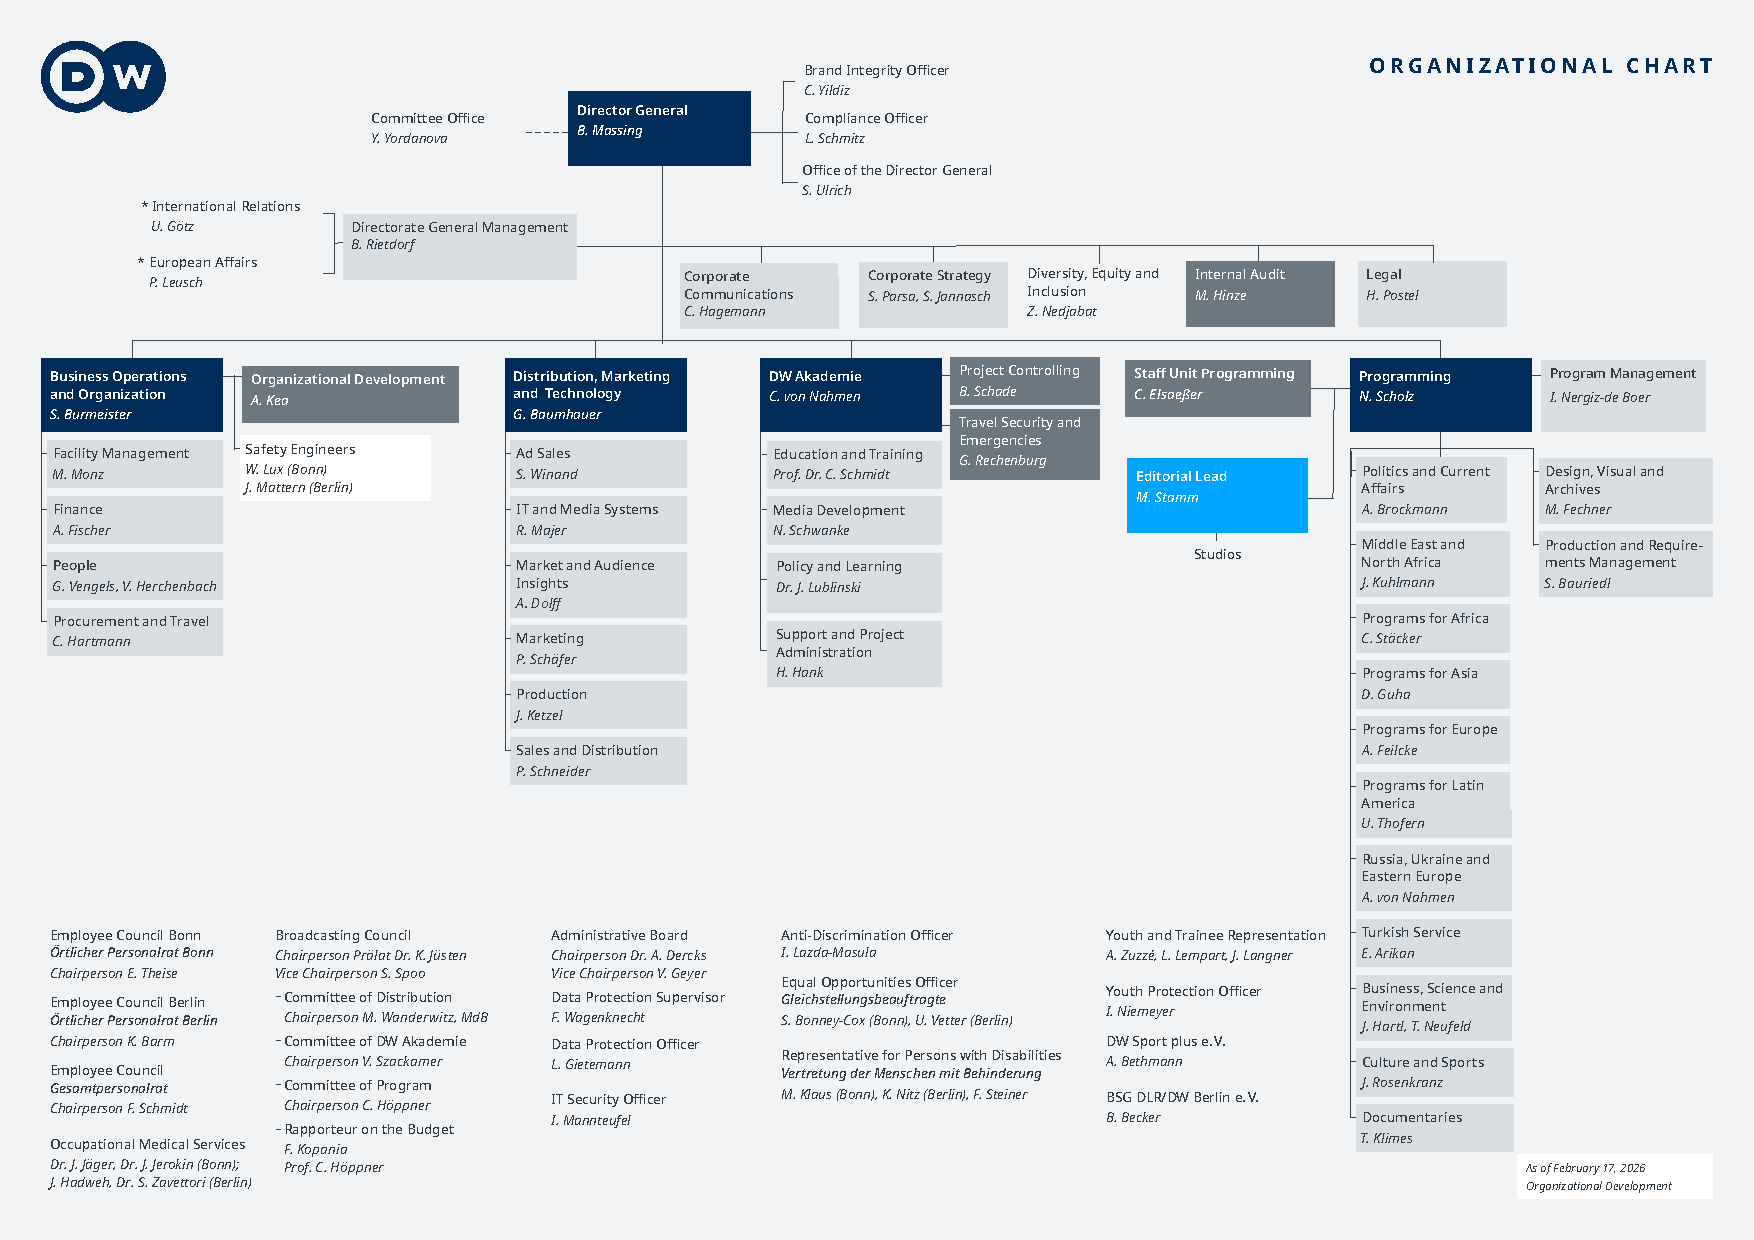
\includegraphics[page=1,width=0.94\textwidth,height=0.38\textheight,keepaspectratio]{Organizational_Chart_Deutsche_Welle.pdf}
\caption{Organisationsübersicht von \companyname{}}
\end{figure}

\subsection*{Relevanter Organisationsausschnitt}
\begin{figure}[H]
\centering
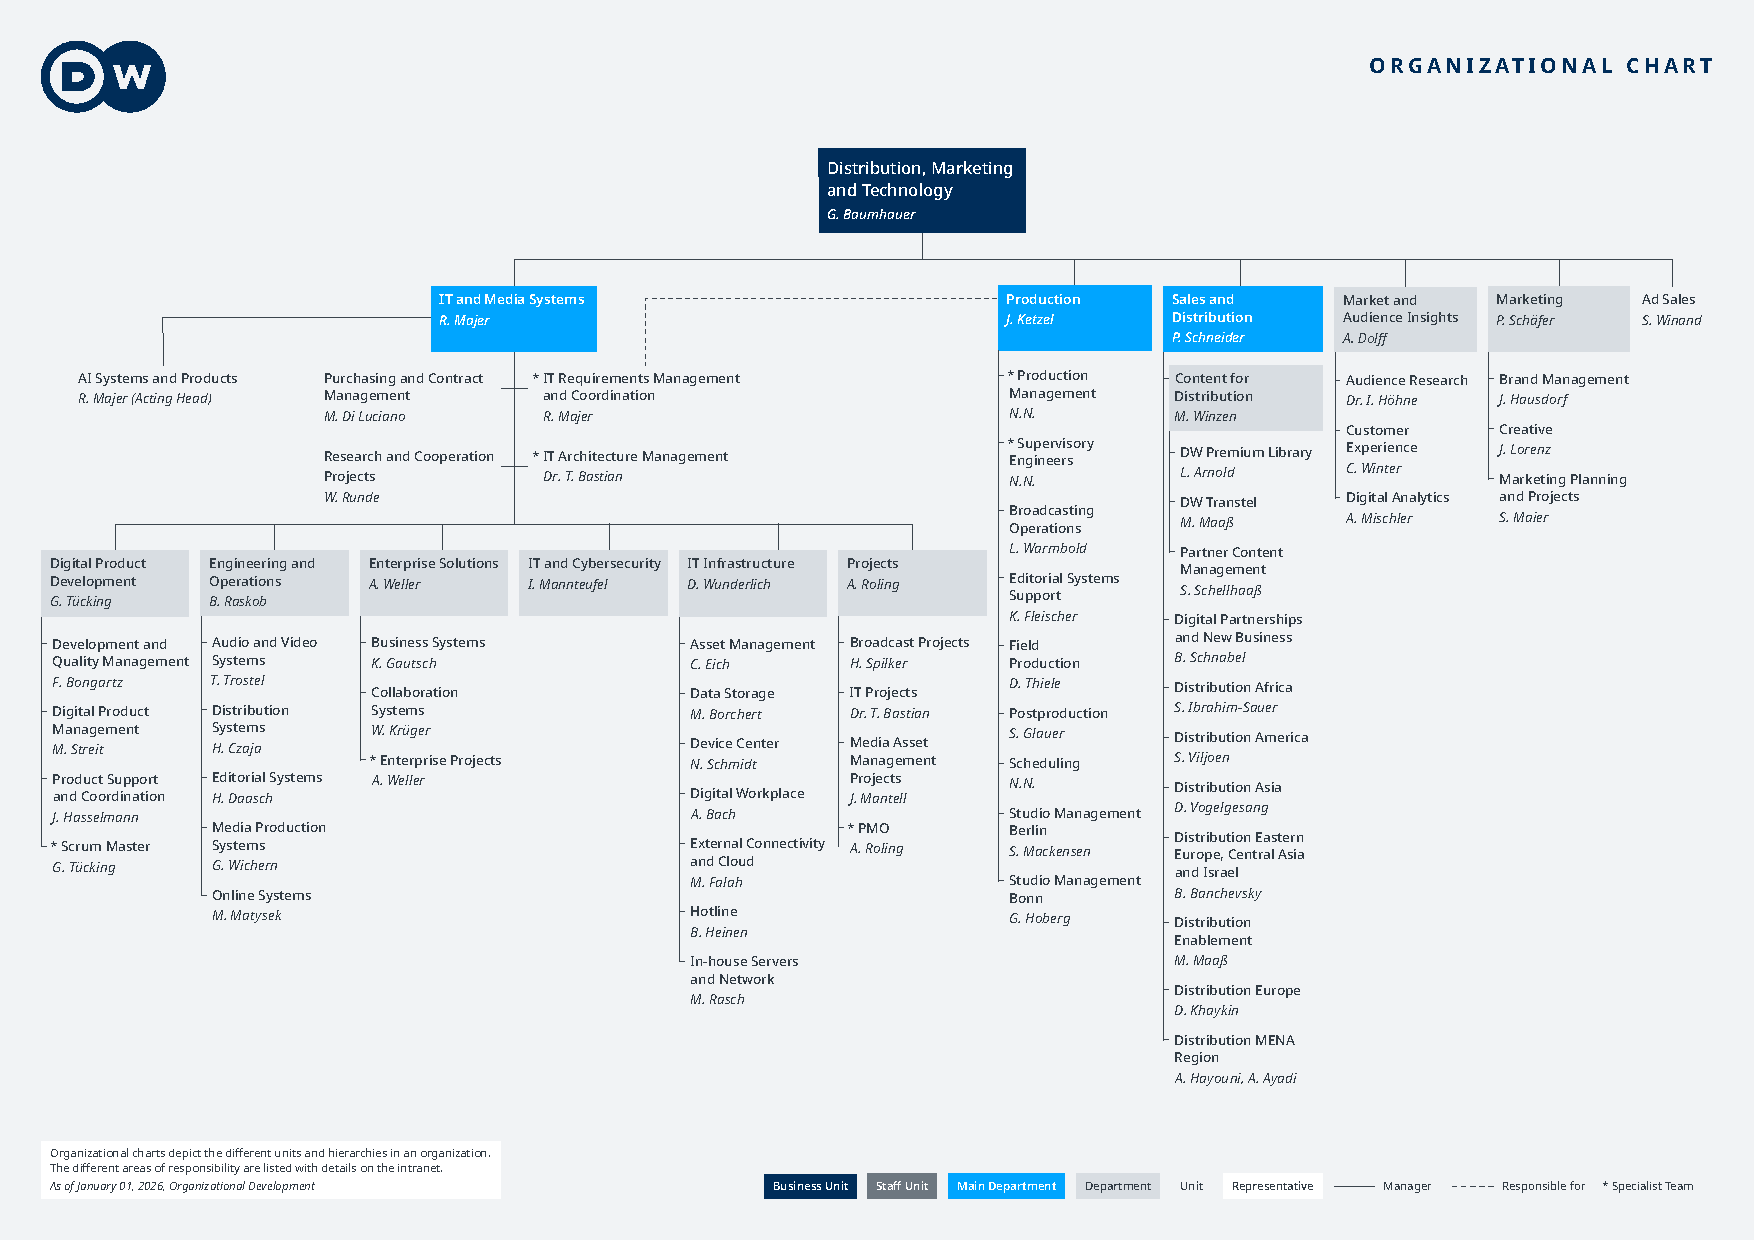
\includegraphics[page=1,width=0.94\textwidth,height=0.38\textheight,keepaspectratio]{Organizational_Chart_Distribution_Marketing_and_Technology.pdf}
\caption{Organisationsausschnitt \emph{Distribution, Marketing and Technology}}
\end{figure}

\clearpage

\section{Prozesslandkarte}
Die Prozesslandkarte unterscheidet Steuerungs-, Kern- und Unterst\"utzungsprozesse. Die
Steuerungsprozesse sind an den Anforderungen eines digitalen Nachrichtenunternehmens ausgerichtet
und fokussieren insbesondere auf publizistische Strategie, Themen- und Publikationsplanung,
Leistungssteuerung, Qualit\"atssicherung sowie regulatorische und ethische Vorgaben. Die
Kernprozesse orientieren sich an der digitalen Medienwertkette nach EBU TR 041v2. Dort wird der
Kern des Medienunternehmens \"uber Prozesse wie \emph{Publication Planning}, \emph{Commissioning},
\emph{Production}, \emph{Publication}, \emph{Distribution}, \emph{User Access}, \emph{User Experience}
und \emph{Analysis} beschrieben.\footnote{Vgl. EBU TR 041v2, \emph{The Digital Media Value Chain},
Figure 9: Core Model, 2024, \url{https://tech.ebu.ch/docs/techreports/tr041.pdf}.}

\begin{figure}[h]
\centering
\resizebox{\textwidth}{!}{
\begin{tikzpicture}[
  x=1cm,
  y=1cm,
  mappentagon/.style={
    signal,
    signal to=east,
    signal from=nowhere,
    draw=none,
    fill=blue!30,
    minimum height=1.55cm,
    minimum width=3.15cm,
    text width=2.7cm,
    align=center,
    font=\bfseries\footnotesize
  }
]
  \draw[black, line width=0.5pt] (0,0) rectangle (21.8,-7.2);
  \draw[black, line width=0.5pt] (0,-2.4) -- (21.8,-2.4);
  \draw[black, line width=0.5pt] (0,-4.8) -- (21.8,-4.8);

  \node[anchor=west, font=\bfseries\large] at (0.25,-0.42) {Steuerungsprozesse};
  \node[anchor=west, font=\bfseries\large] at (0.25,-2.82) {Kernprozesse};
  \node[anchor=west, font=\bfseries\large] at (0.25,-5.22) {Unterstützungsprozesse};

  \node[mappentagon] at (1.95,-1.48) {Audience- und\\Marktstrategie};
  \node[mappentagon] at (5.5,-1.48) {Rechte- und \\Lizenzmanagement};
  \node[mappentagon] at (9,-1.48) {Partner- und\\Kooperationsmanagement};
  \node[mappentagon] at (12.5,-1.48) {Qualitäts-\\sicherung};
  \node[mappentagon] at (16,-1.48) {Medienrecht\\und Ethik};

  \node[mappentagon] at (1.95,-3.88) {Bedarf};
  \node[mappentagon] at (5.5,-3.88) {Publication\\Planning};
  \node[mappentagon] at (9,-3.88) {Commissioning};
  \node[mappentagon] at (12.5,-3.88) {Produktion};
  \node[mappentagon] at (16,-3.88) {Publikation\\und Distribution};
  \node[mappentagon] at (19.5,-3.88) {Analyse};

  \node[mappentagon] at (1.95,-6.28) {Personal\\und Onboarding};
  \node[mappentagon] at (5.5,-6.28) {Beschaffung};
  \node[mappentagon] at (9,-6.28) {Report-\\automatisierung};
  \node[mappentagon] at (12.5,-6.28) {Recht\\und Datenschutz};
  \node[mappentagon] at (16,-6.28) {Finanzen\\und Einkauf};
  \node[mappentagon] at (19.5,-6.28) {IT-\\Plattformbetrieb};
\end{tikzpicture}
}
\caption{Prozesslandkarte von \companyname{}}
\end{figure}

\clearpage
\section{Wertsch\"opfungskettendiagramme}

\textbf{Unterst\"utzungsprozess:} Personal und Onboarding

F\"ur die verfeinerte Betrachtung des Unterst\"utzungsprozesses wird der Bereich
\emph{Personal und Onboarding} dargestellt. Dieser Prozess stellt sicher, dass neue Mitarbeitende
fachlich, organisatorisch und technisch so eingebunden werden, dass sie ihre Aufgaben im
Nachrichtenunternehmen schnell und regelkonform aufnehmen k\"onnen.

\begin{center}
\resizebox{\textwidth}{!}{
\begin{tikzpicture}[node distance=0.38cm]
  \node[wkdstep] (a) {Personalbedarf\\feststellen};
  \node[wkdstep, right=of a] (b) {Stelle\\freigeben};
  \node[wkdstep, right=of b] (c) {Onboarding\\planen};
  \node[wkdstep, right=of c] (d) {Zug\"ange und\\Arbeitsmittel bereitstellen};
  \node[wkdstep, right=of d] (e) {Einarbeitung\\durchf\"uhren};
  \node[wkdstep, right=of e] (f) {Onboarding\\abschlie{\ss}en};
\end{tikzpicture}
}
\end{center}

\vspace{0.8em}
\textbf{Kernprozess:} Analyse

Der ausgew\"ahlte Kernprozess ist der Bereich \emph{Analyse von Inhalts- und Nutzungsdaten}. Er ist Teil der digitalen
Medienwertkette von \companyname{} und beschreibt die Verarbeitung von Inhalts- und
Nutzungsdaten zu steuerungsrelevanten Erkenntnissen und Berichten f\"ur Redaktion, Produkt
und Management.

In diesem Szenario umfasst der Kernprozess Analyse nicht nur die Berechnung und Interpretation
von Kennzahlen, sondern auch die adressatengerechte Aufbereitung der Ergebnisse in Form
interner Berichte. Die eigentlichen Fragestellungen werden dabei in der Regel von anfordernden
Bereichen oder Entscheidungstr\"agern vorgegeben, w\"ahrend die operative Datenauswertung,
Ergebnisinterpretation und Berichtserstellung im Analysebereich erfolgt. Die Berichtserstellung wird
damit nicht als eigenst\"andiger Fremdprozess verstanden, sondern als letzter Schritt des
Analyseprozesses zur Bereitstellung entscheidungsrelevanter Informationen.

\begin{center}
\resizebox{\textwidth}{!}{
\begin{tikzpicture}[node distance=0.38cm]
  \node[wkdstep] (k1) {Analyse-\\anforderung erfassen};
  \node[wkdstep, right=of k1] (k2) {Inhalts- und \\Nutzungsdaten erfassen};
  \node[wkdstep, right=of k2] (k3) {Daten\\aufbereiten};
  \node[wkdstep, right=of k3] (k4) {Datenqualit\"at\\pr\"ufen};
  \node[wkdstep, right=of k4] (k5) {Kennzahlen\\berechnen};
  \node[wkdstep, right=of k5] (k6) {Ergebnisse\\interpretieren};
  \node[wkdstep, right=of k6] (k7) {Berichte\\erstellen};
\end{tikzpicture}
}
\end{center}

\clearpage
\section{BPMN-Diagramm des ausgewählten Kernprozesses}
\begin{figure}[H]
\centering
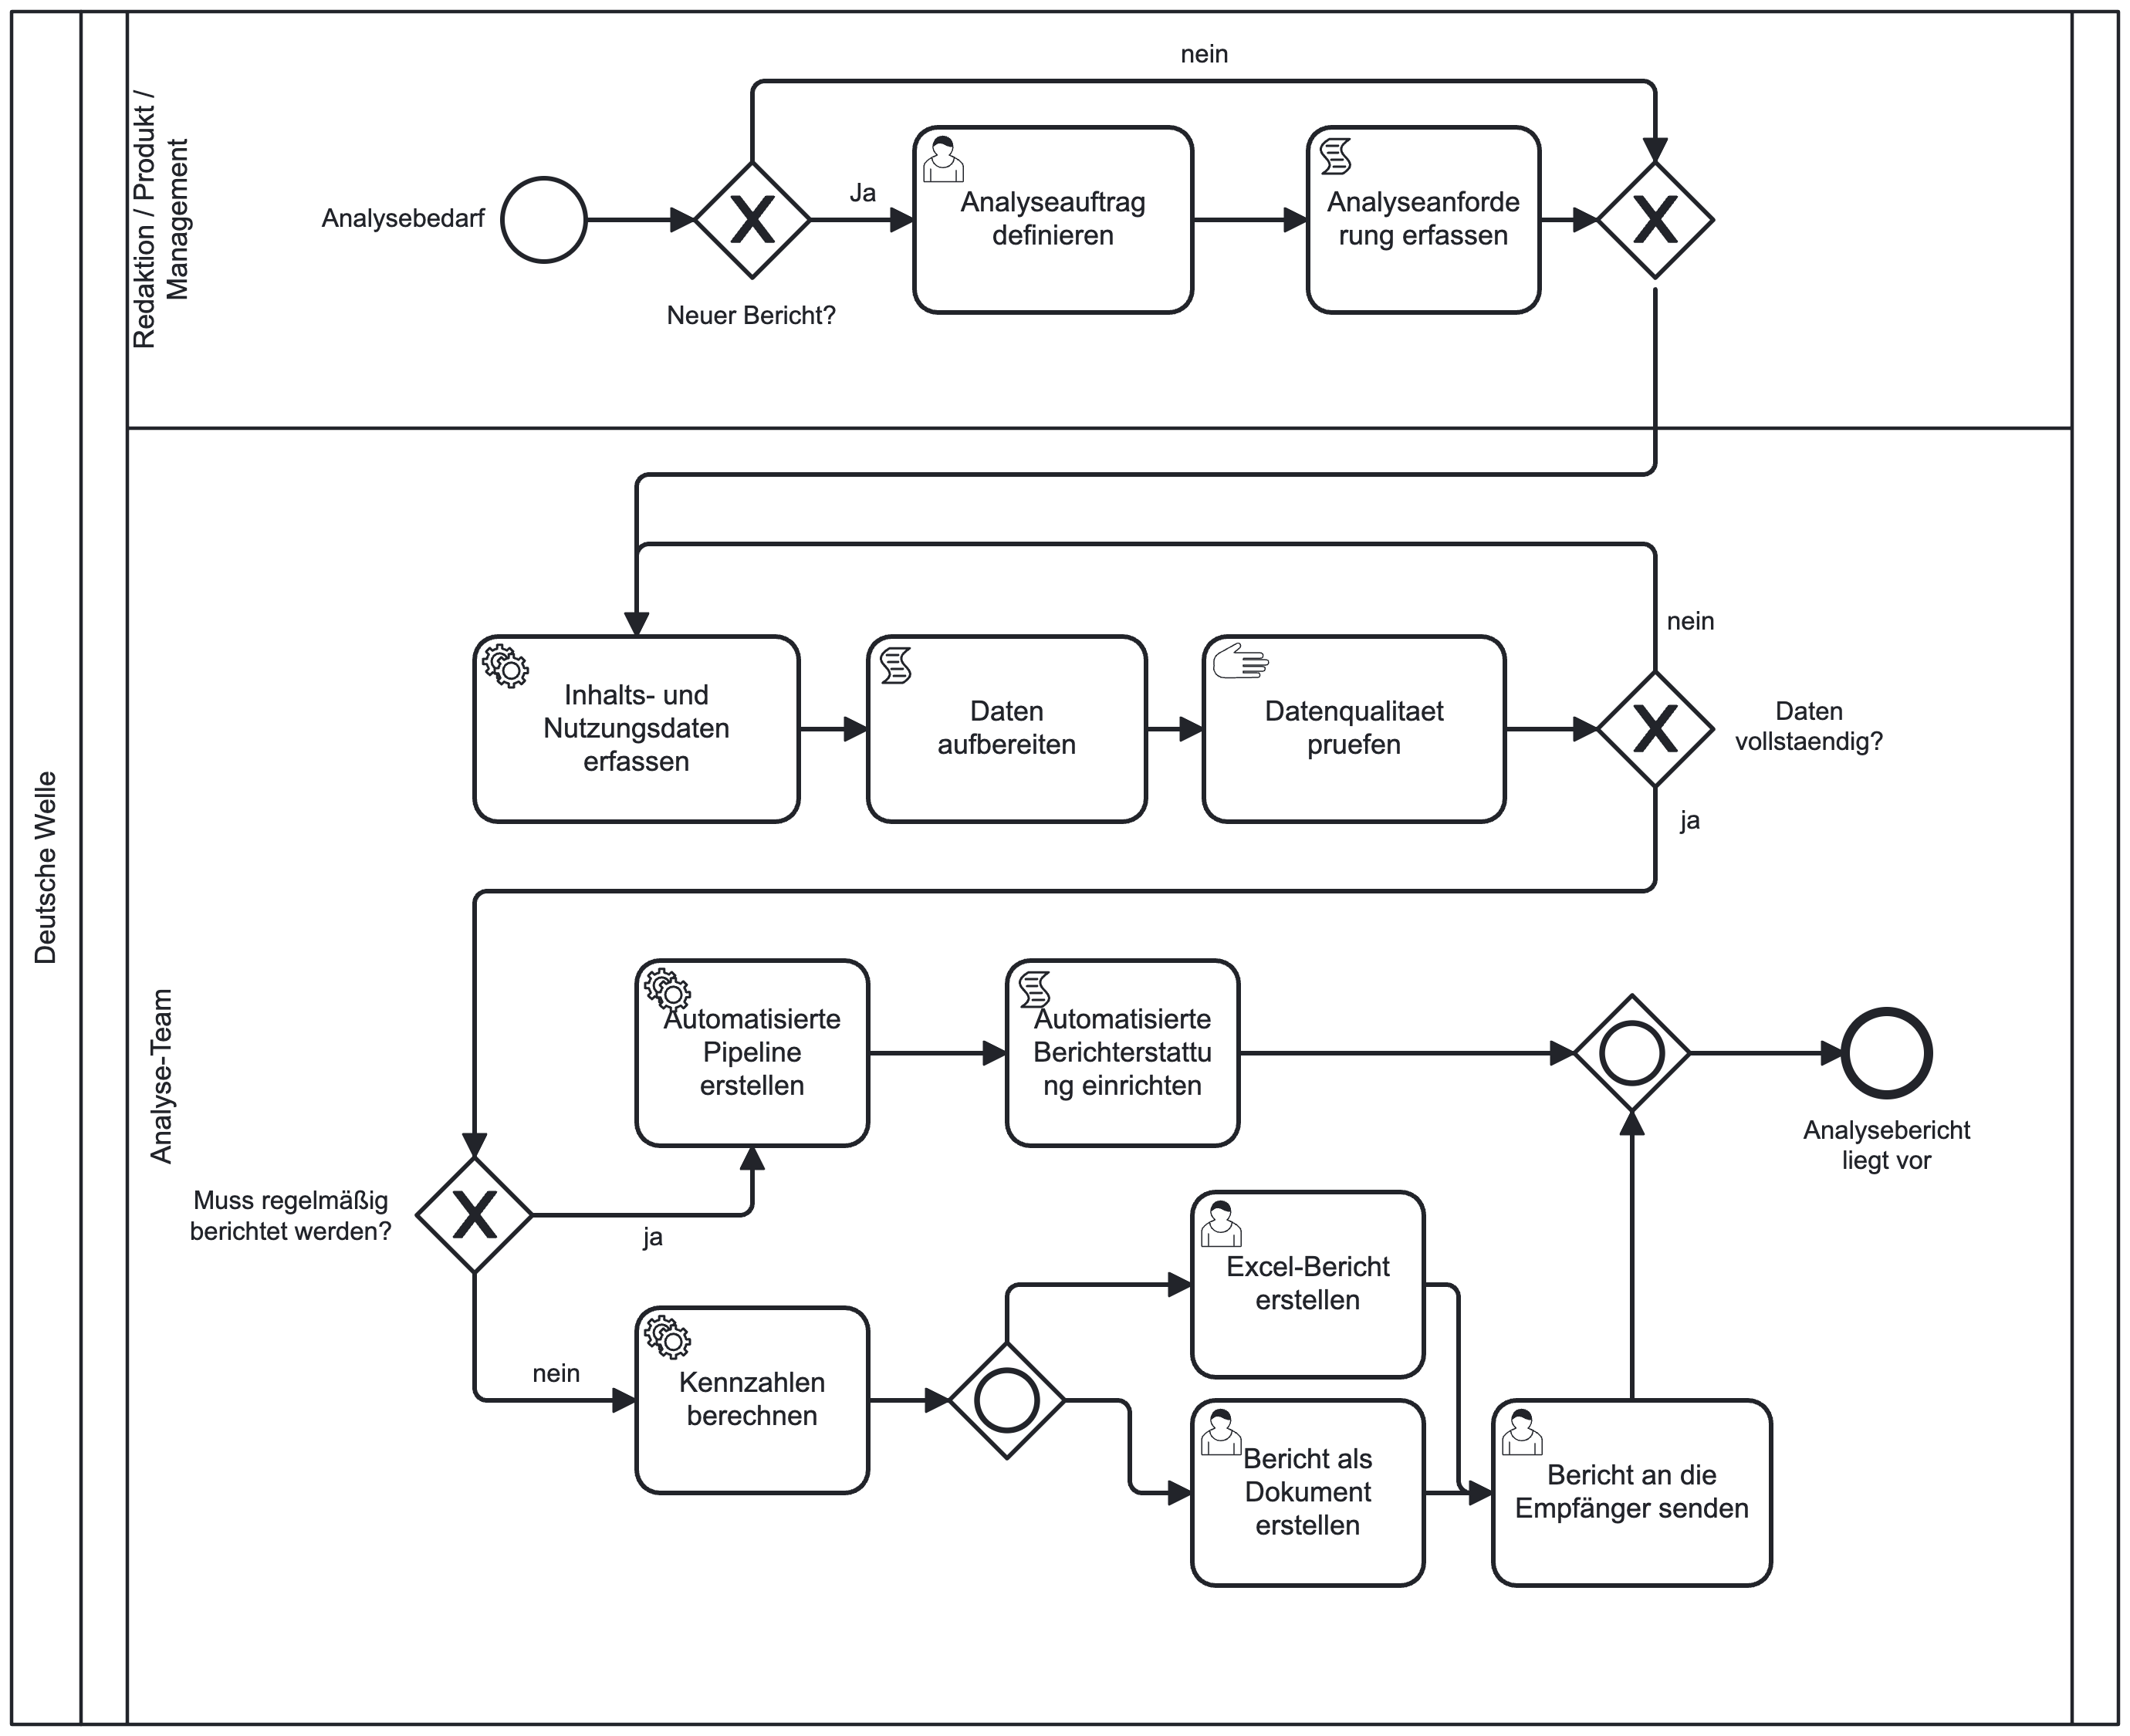
\includegraphics[width=\textwidth]{../bpmn_analyse/bpmn_analyse.png}
\caption{BPMN-nahe Darstellung des Kernprozesses \coreprocess}
\end{figure}

\clearpage
\section{ER-Diagramm für die Entitäten des Unterstützungsprozesses}

\begin{figure}[H]
\centering
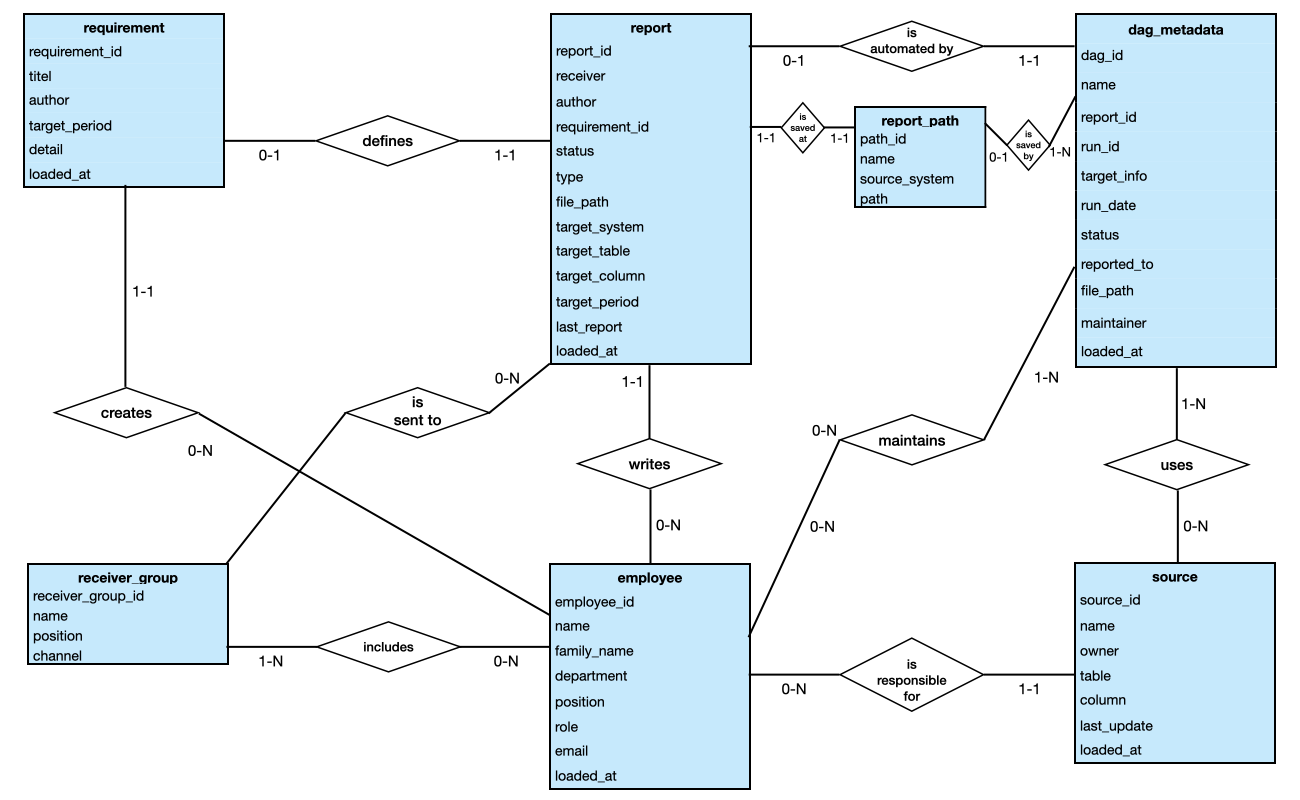
\includegraphics[width=\textwidth]{../er_diagramm/er_diagramm_uncoloured/er_diagramm_uncoloured.001.png}
\caption{ER-Diagramm für den Unterstützungsprozess}
\end{figure}

\section{Konkrete Beschreibung verschiedener Prozessdurchläufe}

\begin{enumerate}
  \item \textbf{Pfad 1: Neuer Bericht, Daten vollständig, regelmäßige Berichterstattung.} Die Chefredakteurin Anna Keller meldet bei dem Analysten Lukas Schneider aus dem Bereich MAI den Bedarf nach einem neuen t\"aglichen Nutzungsbericht an. Die Redaktion m\"ochte vor der Morgenkonferenz jeden Werktag einen konsistenten \"Uberblick \"uber die Entwicklung von Seitenaufrufen, aktiven Nutzerinnen und Nutzern, Verweildauer und Einstiegen nach Plattform erhalten. Lukas definiert mit ihr den Analyseauftrag und erfasst die Anforderungen an Kennzahlen, Empf\"angerkreis und Format. Anschlie{\ss}end organisiert er den Zugriff auf die ben\"otigten Web- und App-Daten, bereitet die Daten auf und stellt bei der Qualit\"atspr\"ufung fest, dass die Datengrundlage vollst\"andig ist. Weil der Bericht an jedem Werktag vor der Morgenkonferenz vorliegen soll, \"ubergibt Lukas die technischen Automatisierungsanforderungen an das Team AIPRO im Bereich ITM. AIPRO richtet die Pipeline und die t\"agliche automatisierte Berichterstattung ein; damit liegt der Analysebericht k\"unftig regelm\"a{\ss}ig vor.

  \item \textbf{Pfad 2: Bestehender Bericht, Daten vollständig, regelmäßige Berichterstattung.} Die Redakteurin Sophie Becker fordert f\"ur den bereits bestehenden w\"ochentlichen Audience-Bericht eine Erweiterung an, weil k\"unftig zus\"atzlich Nutzungsdaten aus dem Newsletter-Kanal ber\"ucksichtigt werden sollen. Die Redaktion m\"ochte nicht nur sehen, welche Inhalte auf Website und App stark genutzt wurden, sondern auch, welchen Beitrag Newsletter-Ausspielungen zur gesamten Reichweite leisten. Die Analystin Lena Hoffmann aus dem Bereich MAI stellt fest, dass kein neuer Bericht angelegt werden muss, sondern der bestehende Bericht angepasst werden kann. Nach der Kl\"arung der Berechtigungen f\"ur die Newsletter-Auswertung werden die Daten erfasst, aufbereitet und erfolgreich auf Vollst\"andigkeit gepr\"uft. Da der Bericht weiterhin w\"ochentlich automatisiert laufen soll, \"ubergibt Lena die \"Anderungsanforderungen an AIPRO, wo die bestehende Berichterstattung technisch angepasst wird.

  \item \textbf{Pfad 3: Neuer Bericht, Daten unvollständig, danach regelmäßige Berichterstattung.} Jonas Weber aus der Wirtschaftsredaktion ben\"otigt einen neuen monatlichen Markt- und Plattformbericht. Die Redaktion m\"ochte \"uber mehrere Monate nachvollziehen, wie sich Zugriffe \"uber Suchmaschinen, Direktzugriffe, soziale Plattformen und Partnerportale entwickeln und ob sich Reichweitenanteile zwischen den Plattformen verschieben. Zusammen mit Lukas Schneider werden Analyseauftrag und Berichtsanforde\-rungen festgelegt. Bei der ersten Datenerfassung zeigt die Qualit\"atspr\"ufung jedoch, dass Daten einer Plattform fehlen. Lukas stimmt sich daher mit dem zust\"andigen Quellsystem-Team ab, l\"asst fehlende Berechtigungen und Datenlieferungen korrigieren und startet die Datenerfassung erneut. Nach erfolgreicher erneuter Pr\"ufung sind die Daten vollst\"andig; anschlie{\ss}end richtet AIPRO die monatliche automatisierte Berichterstattung ein.

  \item \textbf{Pfad 4: Bestehender Bericht, Daten unvollständig, danach regelmäßige Berichterstattung.} F\"ur einen bereits existierenden j\"ahrlichen Strategiebericht fordert Claudia Neumann eine Erweiterung um zus\"atzliche Nutzungsdaten aus einem neuen Video-Kanal auf Connected-TV-Plattformen. Das Management m\"ochte im Jahresr\"uckblick nachvollziehen, wie sich die Nutzung \"uber alle gro{\ss}en Ausspielwege entwickelt hat und ob sich die Gewichte zwischen Website, App, YouTube und Connected TV verschieben. Martin Becker aus dem Bereich MAI behandelt den Vorgang als Anpassung eines bestehenden Berichts. Nach der ersten Aufbereitung zeigt die Datenqualit\"atspr\"ufung, dass die neuen Kanalzahlen noch nicht vollst\"andig geliefert werden. Martin veranlasst gemeinsam mit den Datenverantwortlichen eine Nachlieferung, startet die Erfassung erneut und erh\"alt dann eine vollst\"andige Datengrundlage. Daraufhin wird AIPRO beauftragt, die bestehende j\"ahrliche Berichterstattung technisch zu aktualisieren.

  \item \textbf{Pfad 5: Neuer Bericht, Daten vollständig, bedarfsorientiert, nur Excel-Bericht.} Der Produktmanager Tobias Wagner ben\"otigt kurzfristig eine Auswertung zu einer neuen App-Funktion, bei der Nutzerinnen und Nutzer unter Artikeln einen personalisierten Themen-Feed empfohlen bekommen. Zwei Wochen nach dem Release m\"ochte das Produktteam wissen, ob die Funktion zu mehr Folgeaufrufen pro Sitzung gef\"uhrt hat. Gemeinsam mit der Analystin Julia Hartmann definiert er einen neuen Analyseauftrag und konkretisiert die Anforderungen so, dass vor allem ein Vergleich der Nutzungsverl\"aufe vor und nach dem Release in tabellarischer Form ben\"otigt wird. Nach Datenerfassung, Aufbereitung und erfolgreicher Vollst\"andigkeitspr\"ufung wird entschieden, dass keine regelm\"a{\ss}ige Berichterstattung erforderlich ist. Julia l\"asst die Kennzahlen berechnen; anschlie{\ss}end wird ausschlie{\ss}lich ein Excel-Bericht mit \"Ubersicht und Diagramm erzeugt und an das Produktteam versendet.

  \item \textbf{Pfad 6: Bestehender Bericht, Daten vollständig, bedarfsorientiert, nur Dokumentbericht.} Die Programmplanerin Laura Stein ben\"otigt auf Basis eines bereits bekannten Berichtstyps eine einmalige Auswertung zur Wirkung einer Themenwoche rund um die Fu{\ss}ball-Weltmeisterschaft. W\"ahrend des Turniers wurde f\"ur Fu{\ss}ballartikel erstmals ein Prognose-Format eingef\"uhrt, in dem vor jedem Spiel statistische Vorhersagen und Wahrscheinlichkeiten visualisiert wurden. Laura m\"ochte wissen, ob diese neuen Prognoseartikel h\"ohere Abrufzahlen und l\"angere Verweildauern erzielt haben als klassische Spielvorberichte. Da Struktur und Kennzahlen des Berichtstyps schon existieren, wird kein neuer Bericht angelegt. Nach Datenerfassung, Aufbereitung und erfolgreicher Qualit\"atspr\"ufung wird festgestellt, dass der Bericht nur f\"ur diesen Anlass ben\"otigt wird. Nach der Kennzahlenberechnung wird daher kein Excel-Bericht erzeugt, sondern ausschlie{\ss}lich ein kompakter Dokumentbericht mit eingebetteten Verlaufsdiagrammen erstellt und an Laura Stein sowie die Programmplanung verschickt.

  \item \textbf{Pfad 7: Neuer Bericht, Daten vollständig, bedarfsorientiert, Excel- und Dokumentbericht.} Die Gesch\"aftsleiterin Claudia Neumann fordert f\"ur einen einmaligen Strategie-Workshop einen neuen Analysebericht an, weil \companyname{} nach einem Relaunch der Startseite bewerten m\"ochte, ob sich die Sichtbarkeit internationaler Top-Themen verbessert hat. Gemeinsam mit Martin Becker aus dem Bereich MAI definiert sie die Kennzahlen, Vergleichszeitr\"aume und Empf\"anger. Nach erfolgreicher Datenerfassung, Aufbereitung und Datenqualit\"atspr\"ufung wird entschieden, dass keine regelm\"a{\ss}ige Berichterstattung eingerichtet werden muss. Nach der Kennzahlenberechnung werden sowohl ein Excel-Bericht mit den Detailzahlen als auch ein Dokumentbericht mit Management-Zusammenfassung und Trendvisualisierung erstellt; anschlie{\ss}end werden beide Ergebnisse an die Gesch\"aftsleitung und die relevanten Stakeholder versendet.

  \item \textbf{Pfad 8: Bestehender Bericht, Daten unvollständig, danach bedarfsorientiert, Excel- und Dokumentbericht.} Der Vermarktungsanalyst Felix Braun ben\"otigt kurzfristig einen bestehenden Berichtstyp f\"ur einen monatlichen Kampagnenvergleich in angepasster Form, weil vor einem Sales-Meeting gekl\"art werden soll, wie stark eine gesponserte Klimaserie im Vergleich zu einer gesponserten Innovationsserie performt hat. Zus\"atzlich soll ein Balkendiagramm f\"ur die Pr\"asentation erstellt werden. Julia Hartmann aus dem Bereich MAI behandelt die Anfrage als Anpassung eines vorhandenen Berichtstyps. Bei der ersten Datenqualit\"atspr\"ufung wird jedoch festgestellt, dass Teile der Kampagnendaten fehlen. Nach der Abstimmung mit den verantwortlichen Quellsystemen und einer erneuten Datenerfassung ist die Datengrundlage vollst\"andig. Weil der Bericht nur f\"ur das bevorstehende Meeting ben\"otigt wird, erfolgt keine regelm\"a{\ss}ige Berichterstattung. Nach der Kennzahlenberechnung werden sowohl ein Excel-Bericht als auch ein kurzes Begleitdokument erstellt und an Vermarktung und Audience Insights versendet.
\end{enumerate}

\section{Funktionale Anforderungen}
\begin{itemize}
  \item Das System muss Analyseauftrag und Analyseanforderungen f\"ur neue Berichte erfassen k\"onnen.
  \item Das System muss Inhalts- und Nutzungsdaten aus mehreren Quellen erfassen und aufbereiten k\"onnen.
  \item Das System muss die Datenqualit\"at pr\"ufen und bei unvollst\"andigen Daten eine R\"uckkehr zur Datenerfassung unterst\"utzen.
  \item Das System muss f\"ur regelm\"a{\ss}ige Berichte eine automatisierte Pipeline und eine automatisierte Berichterstattung einrichten k\"onnen.
  \item Das System muss f\"ur bedarfsorientierte Berichte Kennzahlen berechnen sowie Excel-Berichte und/oder Dokumente erzeugen k\"onnen.
\end{itemize}

\end{document}
